\documentclass[tikz,border=4pt]{standalone}
\usepackage[utf8]{inputenc}
\usepackage[T1]{fontenc}
\usepackage{amsmath,amssymb}
\usepackage{lmodern}
\usetikzlibrary{arrows.meta}

\definecolor{ink}{HTML}{1d1d1f}
\definecolor{graytext}{HTML}{515154}
\definecolor{muted}{HTML}{86868b}
\definecolor{amber}{HTML}{ff9f0a}
\definecolor{greenaccent}{HTML}{30d158}
\definecolor{greendark}{HTML}{1a7f37}

\begin{document}
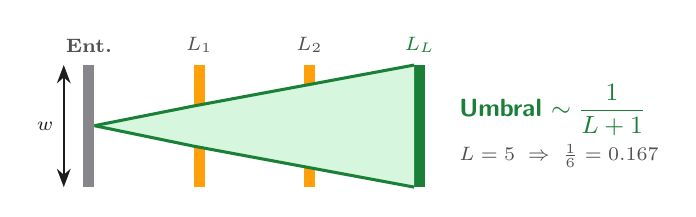
\begin{tikzpicture}[font=\sffamily,>=Stealth]

% Placas verticales
\fill[muted] (0.2,0.1) rectangle (0.34,1.65);
\node[above,font=\scriptsize\bfseries,text=graytext] at (0.27,1.68) {Ent.};

\fill[amber] (1.6,0.1) rectangle (1.74,1.65);
\node[above,font=\scriptsize\bfseries,text=graytext] at (1.67,1.68) {$L_1$};

\fill[amber] (3.0,0.1) rectangle (3.14,1.65);
\node[above,font=\scriptsize\bfseries,text=graytext] at (3.07,1.68) {$L_2$};

\fill[greendark] (4.4,0.1) rectangle (4.54,1.65);
\node[above,font=\scriptsize\bfseries,text=greendark] at (4.47,1.68) {$L_L$};

% Cono acumulado
\fill[greenaccent!20] (0.34,0.88) -- (1.60,0.62) -- (3.00,0.36) -- (4.40,0.10) -- (4.40,1.65) -- (3.00,1.39) -- (1.60,1.13) -- cycle;
\draw[greendark,line width=1.1pt] (0.34,0.88) -- (1.60,1.13) -- (3.00,1.39) -- (4.40,1.65);
\draw[greendark,line width=1.1pt] (0.34,0.88) -- (1.60,0.62) -- (3.00,0.36) -- (4.40,0.10);

% Cota w
\draw[<->,ink,line width=0.8pt] (-0.05,0.10) -- (-0.05,1.65) node[midway,left,font=\scriptsize\bfseries]{$w$};

% Etiqueta de umbral
\node[anchor=west,text=greendark,font=\sffamily\bfseries\small] at (4.85,1.08)
  {Umbral $\sim \dfrac{1}{L+1}$};
\node[anchor=west,text=graytext,font=\sffamily\scriptsize] at (4.85,0.50)
  {$L=5 \;\Rightarrow\; \tfrac{1}{6} = 0.167$};

\end{tikzpicture}
\end{document}
